%!TEX program = xelatex
%!BIB program = bibtex
\documentclass[cn,black,12pt,normal]{elegantnote}
\usepackage{float}
\usepackage{hyperref}
\usepackage{amsmath}
\usepackage{amsfonts}
\usepackage{amssymb}
\usepackage{siunitx}[=v2]
\usepackage{fancyhdr}
\usepackage{newtxtext}
\usepackage{algorithm}
\usepackage{algorithmic}
\newcommand{\uct}[1]{\textsuperscript{\textsuperscript{\cite{#1}}}}
\renewcommand{\tablename}{\textbf{Table}}
\renewcommand{\figurename}{Figure.}
\renewcommand{\refname}{References}
\renewcommand{\contentsname}{Contents}
\renewcommand{\versiontext}{Version: }
\renewcommand{\updatetext}{Update: }
\PassOptionsToPackage{no-math}{fontspec}
\lstset{basicstyle=\footnotesize\ttfamily\color[RGB]{50,0,130},numbers=none,frame=trBL}

\sisetup{mode=text}
\sisetup{range-phrase = \text{ \textasciitilde }}
\pagestyle{fancy}
\fancyhead[L]{School of Software Engineering, Tongji University}
\fancyhead[R]{Data Structure Projects}
\renewcommand{\headrulewidth}{1pt}

\title{Exam Registration\\考试报名系统}
\author{1951510\; 姜文渊}
\institute{\small \url{https://github.com/jwyjohn/Jwy_DataStructureHomework}}
\version{0.50}
\date{\today}

\begin{document}

\maketitle

\textbf{Data structure involved:} Linked list


\tableofcontents

\newpage


\section{Introduction}

Since the 1960s, Computer systems (like mainframes in that time) have long been used to help solving real life problem, other than just doing scientific computation. One type of the common tasks involved in those problems is generally referred to as \textbf{CURD}, which is the shorthand for Create, Update, Retrieve and Delete.

Till today, we have built powerful computer systems, both hardware and software, to tackle with the ever increasing need for fast and robust CURD tasks. Examples of the STATE OF THE ART systems are various database systems used in banks, governments and service providers, which holds tetra bytes of records and process thousands of CURD commands in a second, without a single error the whole year. Most of these systems are based on B-trees\uct{bayer1970textordfeminineorganization}, but in recent yaers, more models and algorithms on this topic emerges.

But to a system that need to hold only thousnad of records, the simple data structure, \textbf{linked list}, could meet the need on modern hardware, and the author implemented the system using linked list.

\section{Demostration}

\subsection{Compile and run the program}

On linux platform with \lstinline{make} and a \lstinline{g++} which supports C++ 11 Standard, just \lstinline{cd} to the \lstinline{./linux} and run \lstinline{make build}. The binary executable will be generated in the same dirctory named as \lstinline{a.out} or \lstinline{exam}, according to the configurations in the \lstinline{Makefile}. Use \lstinline{./a.out} or \lstinline{./exam}to run the program.

The program is an interactive shell, where you can input commands and get results.

\begin{figure}[H]
    \centering
    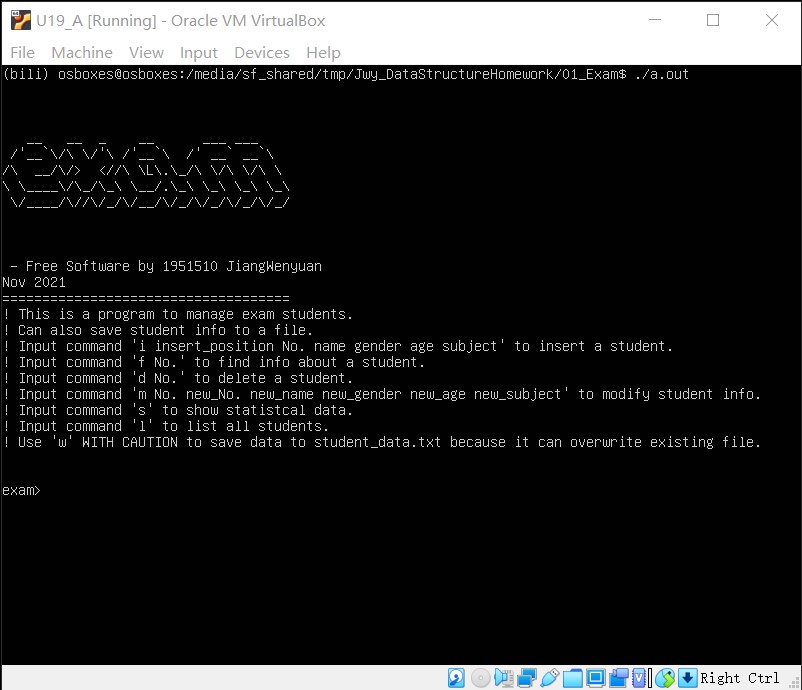
\includegraphics[width=0.7\linewidth]{image/exam_01.jpg}
    \caption{The user interface of the program}
\end{figure}

Usage of commands can be found on the main screen, and the \lstinline{help} command can give you information about theses commands.  All available commands is listed below.

\begin{enumerate}
    \item \lstinline{help} : Show help for a certain command.
    \item \lstinline{exit} : Exit the program.
    \item \lstinline{i [insert_position] [No.] [name] [gender] [age] [subject]} : Insert a candidate to the table, with \lstinline{[insert_position] [No.] [name] [gender] [age] [subject]} given.
    \item \lstinline{f [No.]} : Find a candidate with certain No.
    \item \lstinline{d [No.]} : Delete a candidate with certain No.
    \item \lstinline{m [No.] [new_No.] [new_name] [new_gender] [new_age] [new_subject]} : Modify a candidate with the \lstinline{[new_No.] [new_name] [new_gender] [new_age] [new_subject]}.
    \item \lstinline{l} : List all information of the candidates.
    \item \lstinline{s} : Show statistical data of the candidates.
    \item \lstinline{w} : Write the candidates' information to a file.
\end{enumerate}

\subsection{Add candidates to the table}

Type \lstinline{i [insert_position] [No.] [name] [gender] [age] [subject]} to add some candidates. Then use \lstinline{l} to list all the candidates added.

\begin{figure}[H]
    \centering
    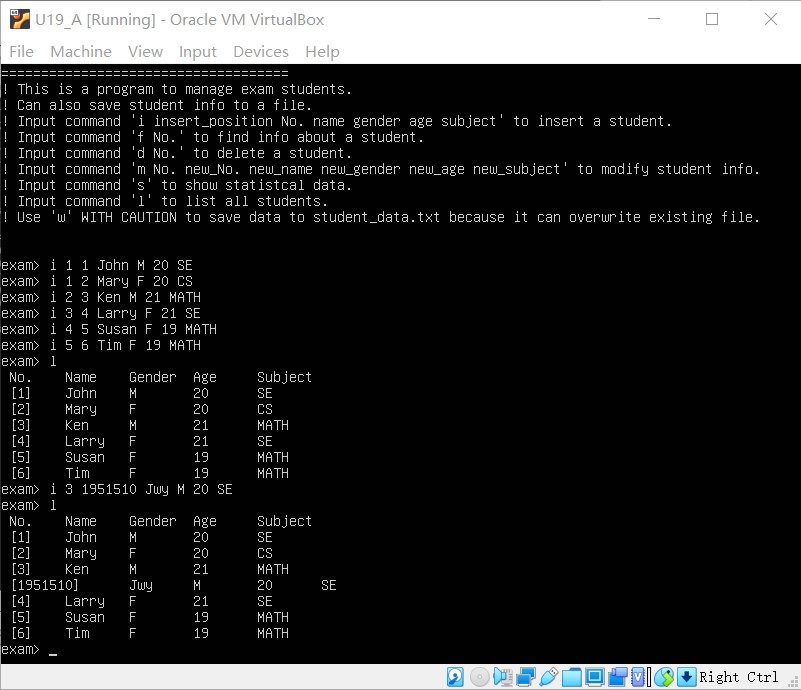
\includegraphics[width=0.7\linewidth]{image/exam_02.jpg}
    \caption{Add candidates to the table and view them}
\end{figure}

\subsection{Manage candidates}

\begin{figure}[H]
    \centering
    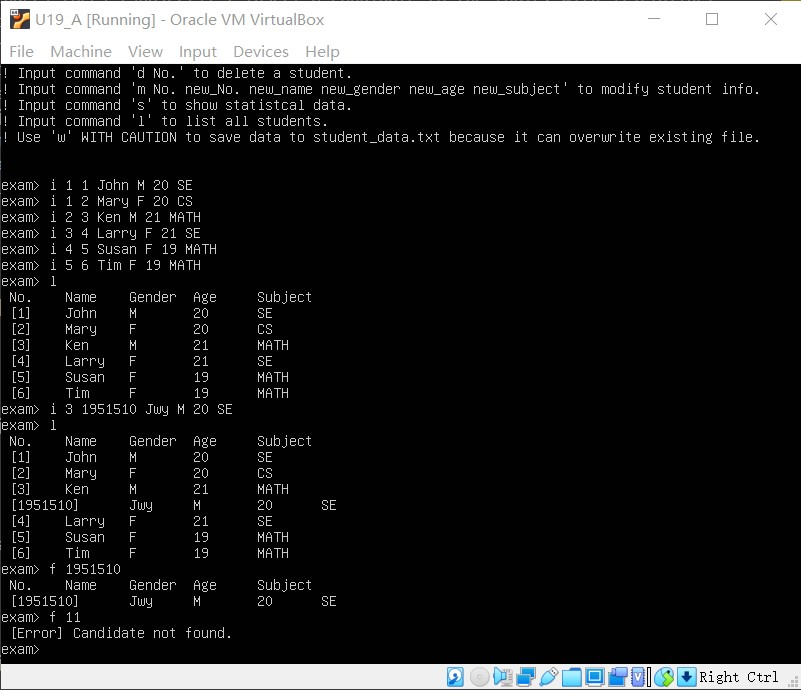
\includegraphics[width=0.7\linewidth]{image/exam_03.jpg}
    \caption{Use \lstinline{f [No.]} to find a candidate}
\end{figure}
To find a candidate, use \lstinline{f [No.]}. In this case, we want to find 1951510 in the table, so just type \lstinline{f 1951510} in the console. We also want to try what could happen if a candidate is not in the table, so we used \lstinline{f 11}. The program then prints out the information about the students, if it has found them, as is shown on the figure above.

Then the removal and modification of the candidates can be done using the commands in the previous subsections. For example, we want to remove the candidate with No. 1951510, and correct the No. of Tim to 7, and the gender of him to Male, and change his subject to SE.

Note that if a user inputs invalid commands or arguments, the program will be robust enough (at least to some extent) to detect the exception and return an error message. Detailed Demostration of this feature can be explored when using this program.

\begin{figure}[H]
    \centering
    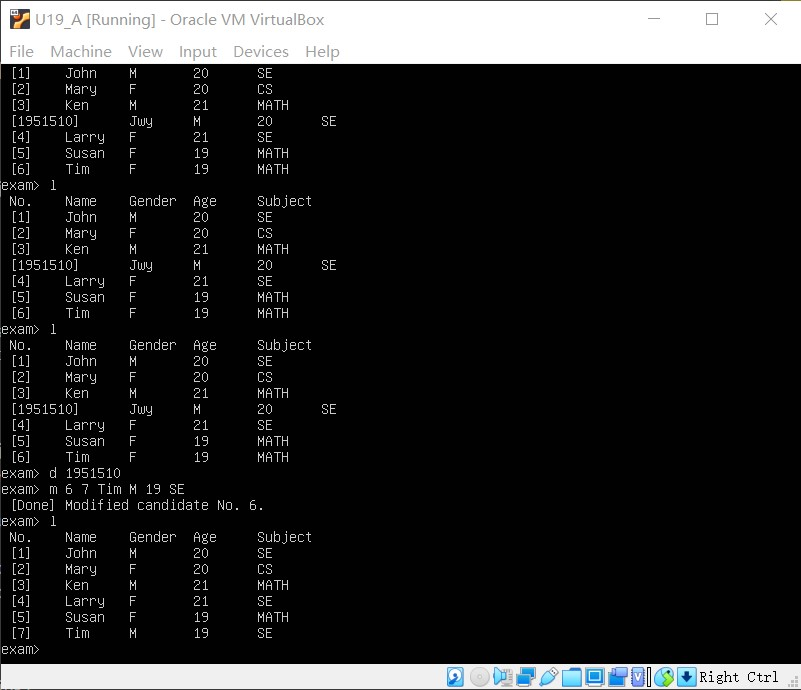
\includegraphics[width=0.7\linewidth]{image/exam_04.jpg}
    \caption{Manage the candidates}
\end{figure}

\subsection{Do some statistics}

The program also support doing some simple statistical analysis to the candidates, try \lstinline{s}.

As can be seen in the figure below, the number of candidates of different age, gender and subject are counted, for a better overview of the candidate group.

\begin{figure}[H]
    \centering
    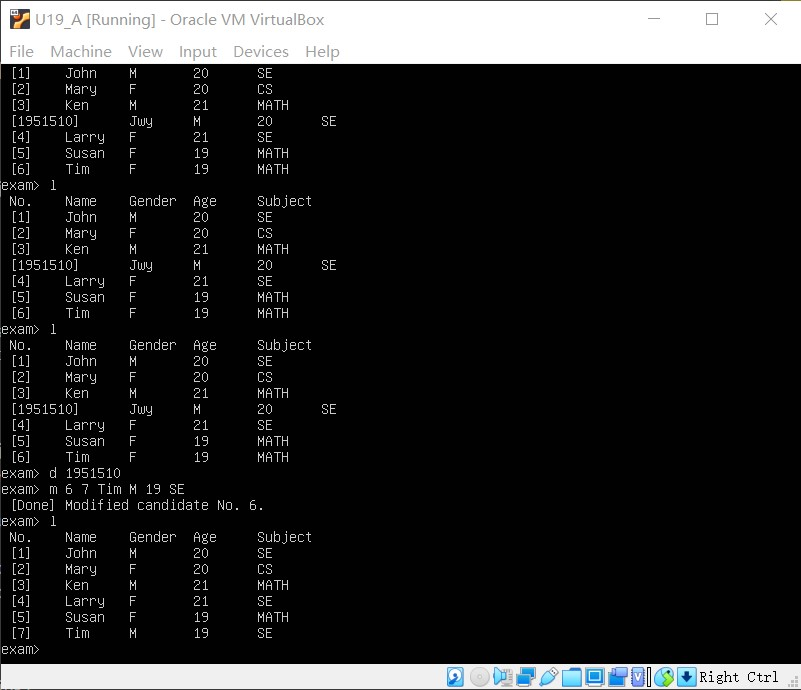
\includegraphics[width=0.7\linewidth]{image/exam_05.jpg}
    \caption{Do some statistics}
\end{figure}

\subsection{Save the data}

Type \lstinline{w} to write the table to the file \lstinline{student_data.txt}, which looks like this:
\begin{lstlisting}[language = C++]
i 1 1 John M 20 SE
i 1 2 Mary F 20 CS
i 2 3 Ken M 21 MATH
i 3 4 Larry F 21 SE
i 4 5 Susan F 19 MATH
i 5 7 Tim M 19 SE
\end{lstlisting}
This file stores commands to import the table into the program, just copy and paste them into the console, and the data will be the same as before.

\begin{figure}[H]
    \centering
    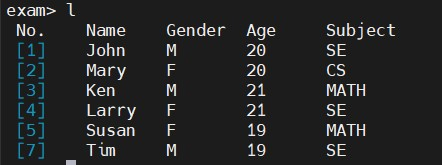
\includegraphics[width=0.5\linewidth]{image/exam_06.jpg}
    \caption{The imported data from another console}
\end{figure}

\section{About linked list}

Linked list is a data structure consisting of a collection of nodes with pointers onto their next node, which together represent a sequence. A simple figure below can demostrate the basic features of a linked list. \uct{wiki:Linked_list}

\begin{figure}[H]
    \centering
    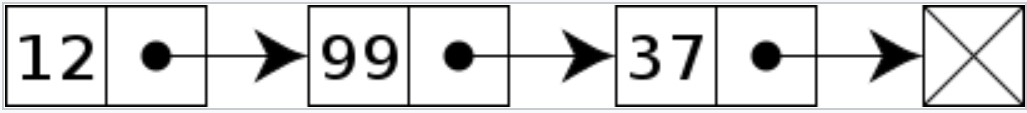
\includegraphics[width=1.0\linewidth]{image/ll_01.jpg}
    \caption{A simple diagram showing a \textbf{Singly linked list} (diagram produced by Lasindi)}
\end{figure}

There are several improvements on this data structure. For example, \textbf{Doubly linked list} which has a second link field pointing to the 'previous' node in the sequence for every node, which makes the visit to \lstinline{a[i-1]} from \lstinline{a[i]} much faster.

\begin{figure}[H]
    \centering
    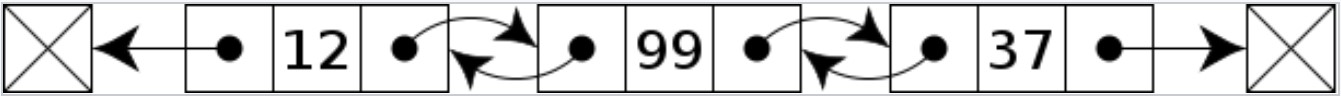
\includegraphics[width=1.0\linewidth]{image/ll_02.jpg}
    \caption{A simple diagram showing a \textbf{Doubly linked list} (diagram produced by Lasindi)\uct{wiki:Linked_list}}
\end{figure}

Another well-known variant of the Singly linked list is the \textbf{Circular linked list}, whose 'last' node points to its 'first' node, as is shown in the figure below.

\begin{figure}[H]
    \centering
    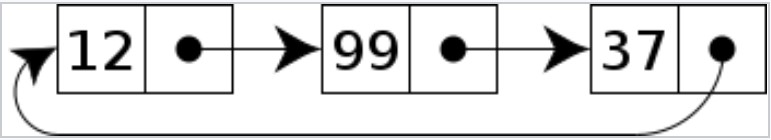
\includegraphics[width=1.0\linewidth]{image/ll_03.jpg}
    \caption{A simple diagram showing a \textbf{Circular linked list} (diagram produced by Lasindi)\uct{wiki:Linked_list}}
\end{figure}


Compared with many other data structures used to maintain a sequence, Linked list is fairly fast on the insertion and deletion operation ($O(1)$ if a pointer to the element that needs to be operated is given). However, the search operation is much slower than most other data structures, making linked list a quick-and-dirty implementation of some needs.

The detailed comparasion is shown in the table below.

\begin{table}[H]
    \caption{\textbf{Comparison of linked list with other data structures}}
    \centering
    \begin{tabular}{cccccc}
        \toprule
        Data structure    & Search       & Insert or Delete     & Excess space  \\
        \midrule
        Linked list       & $O(n)$       & Search time + $O(1)$ & $O(n)$        \\
        Array             & $O(1)$       & $O(n)$               & $O(1)$        \\
        Balanced tree     & $O(log\, n)$ & $O(log\, n)$         & $O(n)$        \\
        Hashed array tree & $O(1)$       & $O(1)$               & $O(\sqrt{n})$ \\
        \bottomrule
    \end{tabular}
\end{table}

As can be seen in the table, linked list performs poorly nearly in all aspects, but is you look at the Line of Code (LOC) for implementation of each algorithm, it turns out that linked list are the winner, which costs less than 50 LOC to implement. The following data comes mainly from Github repo \url{https://github.com/xtaci/algorithms}.

\begin{table}[H]
    \caption{\textbf{Comparison of linked list with other data structures}}
    \centering
    \begin{tabular}{c|cccc}
        \toprule
        Data structure & list      & avl tree   & rb tree               & hash table \\
        \midrule
        LOC            & <50 lines & 243 lines & 187 lines + 264 lines & 160 lines  \\
        \bottomrule
    \end{tabular}
\end{table}

Thus the advantage of linked lists lies not in its performance, but in its simplicity. On most ordinary situations in our PC machine, need for dealing with massive data rarely happens, so even in an operating system (some version of Unix for example\uct{bach1986design}), linked lists are widely used to maintain references to active processes, threads, and other dynamic objects.\uct{wiki:Linked_list}


\section{Notes on the source code}

If you want to modify or re-use the author's code, here are some explaination about the important part of the code. Comments in the source file can provide detailed help, but the following shows the outline.

The node of a linked used in this project is defined here:
\begin{lstlisting}[language = C++]
struct exam_candidate
{
    ... Data of candidates ...
    exam_candidate *next = NULL;
    exam_candidate *pre = NULL;
};
\end{lstlisting}
which is a Doubly linked list with \lstinline{*next} and \lstinline{*pre}.

Operations of the linked list involves several functions:
\begin{lstlisting}[language = C++]
int init_link();
exam_candidate *find_candidate(int no);
int insert_candidate_after(int no, exam_candidate *candidate);
int remove_candidate(int no);
int show_candidates();
int show_single_candidate(exam_candidate *candidate);
\end{lstlisting}

The algorithms used to maintain the linked list follows the description in the textbooks, for example:
\begin{lstlisting}[language = C++]
exam_candidate *find_candidate(int no)
{
	exam_candidate *ptr = head;
	if (no == 0)
		return ptr;
	while (ptr->next != NULL)
	{
		ptr = ptr->next;
		if (ptr->No == no)
			return ptr;
	};
	return NULL;
};
\end{lstlisting}
The \lstinline{find_candidate} function is a standard way of searching in a linked list, and the same is true for insertion:
\begin{lstlisting}[language = C++]
int insert_candidate_after(int no, exam_candidate *candidate)
{
	exam_candidate *insert_position = find_candidate(no);
	if (insert_position == NULL)
		return 0;
	if (insert_position->next != NULL)
	{
		exam_candidate *tmp = insert_position->next;
		insert_position->next = candidate;
		candidate->pre = insert_position;
		candidate->next = tmp;
		tmp->pre = candidate;
	}
	else
	{
		insert_position->next = candidate;
		candidate->pre = insert_position;
	};
	return 1;
};
\end{lstlisting}

Note that most of the code in \lstinline{main.cpp} is for processing the user's input, which is not so interesting.

\section{Discussion}

Even though the performance of Doubly linked list is not excellent, there are still some tricks in optimizing the data structure. One of the direct improvements on liked list is \textbf{XOR linked list}.

For a Doubly linked list with $n$ elements, we usually need to store $2n$ pointers, but a trick called \textbf{XOR linked list} can reduce the amount $2n$ to $n$. \uct{lewin2012all}

\begin{lstlisting}
....A     B         C         D       E ....
    <–>  A^C  <->  B^D  <->  C^E  <->
\end{lstlisting}
The \lstinline{link} field of each node is now \lstinline{pre^next}. We store the pointer to last visted node, and when we want to visit the next node, we could just use \lstinline{last^link} as the \lstinline{next} pointer. The same is ture when visiting backwords.
For example, when we are now at \lstinline{B}, the pointer of \lstinline{C} can be calculated using \lstinline{A^(A^C) = C}.

\bibliography{references}
\end{document}
